\documentclass{beamer}

\usepackage{biblatex} %Imports biblatex package
\usepackage{amsmath}
\addbibresource{bibliografia.bib} %Import the bibliography file


%Information to be included in the title page:
\title{ISPR Mid Term 4:\\Trust Region Policy Optimization}
\author{Luca Moroni\\Mat: 635966}
\institute{ISPR}
\date{2022}

\usetheme{AnnArbor}

\begin{document}

\frame{\titlepage}

\begin{frame}
\frametitle{Introduction}
In a Reinforcement Learning Scenario the policy optimization methods are those technique used to optimize the policy, or rather the probability distribution over possible actions given a state ($\pi(a, s)$).\\~\\
The work described in \cite{schulman2015trust} introduce a method for policy optimization (learns a parametrized policy), defining a policy gradient method similar to the natural policy gradient one.\\~\\
The \textbf{Natural policy gradient methods} want to change the parameters of the policy ($\theta_{old} \to \theta_{new}$) without changing to much the relative distributions $\pi_{\theta_{old}}$,  $\pi_{\theta_{new}}$.
\end{frame}

\begin{frame}
\frametitle{Model Description}
Let $\pi$ a policy, the following identity is an approximation (simpler to optimizer w.r.t the exact one) of the expected return of another policy $\hat{\pi}$ in terms of the advantage over $\pi$.\\
\[L_{\pi}(\hat{\pi}) = \eta(\pi) + \sum_s \rho_{\pi}(s) \sum_a \hat{\pi}(a,s) A_{\pi}(s,a)\]
Where $\eta$ is expected discounted reward, $\rho_{\pi}$ is the discounted visitation frequencies and $A_{\pi} = Q_{\pi}(s, a) - V_{\pi}(s)$ is the advantage function.\\
The following statement hold for any $\theta_0$,
\[\nabla_{\theta} L_{\pi_{\theta_0}} (\pi_{\theta}) (\theta_0) = \nabla_{\theta} \eta (\pi_{\theta}) (\theta_0)\]
So, a suffcient small step ($\pi_{\theta_0} \to \hat{\pi}$) that improve $L_{\pi_{\theta_{0}}}$ will improve $\eta$.
\end{frame}

\begin{frame}
\frametitle{Model Description (II)}
Can be defined a class of methods calld minorization-maximization (MM) that iterativelly (moving from $\pi_{old} \to \pi_{new}$) try to push up the L factor. Those kind of methods works for general definition of $\pi$ (we are in a situation in which $\pi$ is parametrized by a vector $\theta$) and cannot handle large updates, so in \cite{schulman2015trust} it is defined the TRPO method that find the new policy solving the following maximization problem,
\begin{gather*}
maximize_{\theta} \; L_{\theta_{old}}(\theta)\\
subject \, to \; D_{KL}^{\rho_{\theta_{old}}} (\theta_{old}, \theta) \leq \delta.
\end{gather*}
Where $D_{KL}^{\rho_{\theta_{old}}}$ is the average KL divergence.
\end{frame}

\begin{frame}
\frametitle{Model Description (III)}
In \cite{schulman2015trust} is also stated how the objective function and the constraint, of the just showed optimizations problem, can be approximated using Monte Carlo simulation.
\begin{itemize}
    \item \textbf{single path}: sampling individual trajectories.
    \item \textbf{vine}: construct a rollout set, performing multiple actions from each state in teh rollout set.
\end{itemize}
\end{frame}

\begin{frame}
\frametitle{Key catch (I)}
The key catch of the model described until now is the principled methodologies applied in the minorization-maximization (MM) algorithm, from which is derived the TRPO methodology.
Algorithm 1 from \cite{schulman2015trust}.\\~\\
\begin{centering}
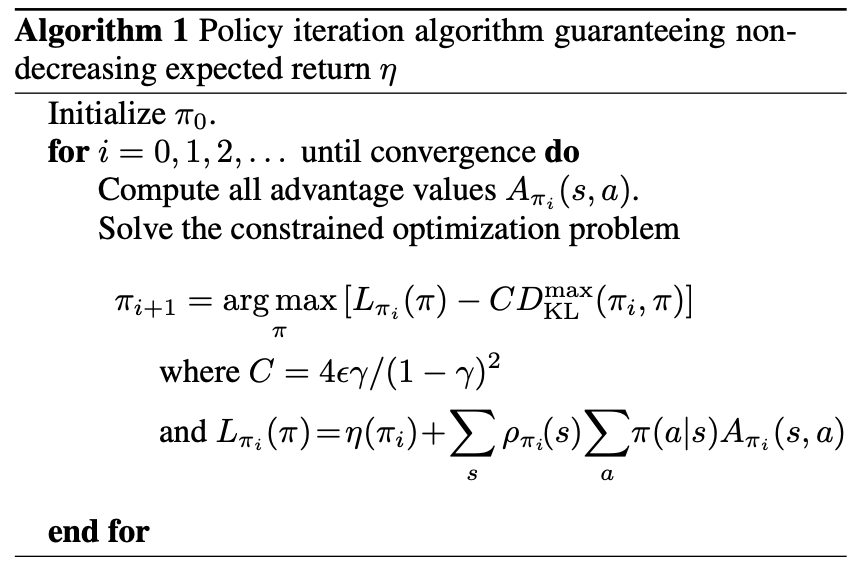
\includegraphics[width=7cm]{algo.png}\\
\end{centering}
\end{frame}

\begin{frame}
\frametitle{Key catch (II)}
As a corollary of the Theorem1 in \cite{schulman2015trust} hold that,
\begin{gather*}
\eta(\hat{\pi}) \geq L_{\pi}(\hat{\pi}) - C \, D_{KL}^{max}(\pi, \hat{\pi}),\\
where \; C = \frac{4\epsilon\gamma}{(1-\gamma)^2}, \\
and \; D_{KL}^{max}(\pi, \hat{\pi}) = \max_s D_{KL}(\pi(\cdot|s) \, \| \, \hat{\pi(\cdot|s)}).
\end{gather*}
From that equation the policies generated from the MM algorithm are monotonically improving w.r.t $\eta$.
Let $M_i(\pi) = L_{\pi_i}(\pi) - C \, D_{KL}^{max}(\pi_i, \pi)$, then $\eta(\pi_{i+1}) - \eta(\pi_i) \geq M_i(\pi_{i+1}) - M_i(\pi_{i})$, maximizing $M_i$ at each iteration, $\eta$ is non-decreasing.\\
TRPO derive from this methodoligy, specifying the $\pi$ for the vectorized parametrized ones, taking out the $-C \, D_{KL}^{max}(\pi, \hat{\pi})$ factor from the objective and use an heuristic approximation of it in the constraint.
\end{frame}

\begin{frame}
\frametitle{Results}
The method described so far was tested over tree high dimensional models of locomotion controller (hard problem), compared with other methods of gradient-free type and natural policy nature, TRPO outperforms all of them.\\
TRPO can do well even in the case of playing Atari games (using CNN with tens of thousand of parameters), even in this case the TRPO based method can do very well.\\
The results in \cite{schulman2015trust} demonstrate good generalization property, since there aren't used engeneered policy, no locomotion notion inside the policy used for TRPO, and no engeenered features in the case of Atari game playing as in other methods.
\end{frame}

\begin{frame}
\frametitle{Comments}
As demonstrated by the empirical results this method can do very well in high dimensional problem without having prior knowledges. Moreover TRPO is a method derived by a principled approach that is rearranged, in a formal way, to deal with some unpractice numerical limitations given by the previous methods, such as small steps in MM. To the other hand in \cite{schulman2015trust} is ignored the estimation error for the advantage function ($A_{\pi}$) so a deeper study on this fact could be done but was omitted for simplicity by the authors.
\end{frame}

\begin{frame}
\frametitle{Bibliography}
\printbibliography
\end{frame}

\end{document}

